\documentclass[conference]{IEEEtran}
\IEEEoverridecommandlockouts
% The preceding line is only needed to identify funding in the first footnote. If that is unneeded, please comment it out.
\usepackage{cite}
\usepackage{amsmath,amssymb,amsfonts}
\usepackage{graphicx}
\usepackage{textcomp}
\usepackage{xcolor}
\def\BibTeX{{\rm B\kern-.05em{\sc i\kern-.025em b}\kern-.08em
    T\kern-.1667em\lower.7ex\hbox{E}\kern-.125emX}}
\title{
\vspace{1cm}
{
\includegraphics[width=0.15\textwidth]{ /storage/emulated/0/vignan/IMG-20241018-WA0001.jpg} \\ Avr-Gcc Assignment}}
\author{Bynaboyina Aiswarya \\ Roll No: FWC22295 \\ aiswaryabaiswarya61@gmail.com}
 \begin{document}
\maketitle
 \section{ABSTRACT}

 This paper explains about the question tests the validity of Boolean identities involving the XOR $(\oplus)$ operator. Four expressions are given, and the objective is to identify which one does not represent a valid identity. The provided options explore properties such as associativity, distributivity, and specific conditions for XOR operations.
\begin{enumerate}
\item  $(x \oplus y) \oplus
 z = x  \oplus (y \oplus z) $ 
\item  $(x + y)  \oplus z = x  \oplus
  (y + z)$
\item  $ x \oplus y = x + y, if xy=0 $
\item  $ x \oplus y = ( xy +x'y' )' $
\end{enumerate}
The question can be implemented using avr-gcc with arduino uno and led.

\section{COMPONENTS} 

The required components list is given in Table: I., pin diagram of Led is shown in Fig.1.
\vspace{0.1cm}
 \begin{table} [htbp]
\centering
\begin{tabular}{| c | c | c |} \hline
Components & Value & Quantity \\\hline
Arduino & UNO & 1 \\ \hline
led &  & 1 \\ \hline
Jumper Wires &  & 20 \\ \hline
Breadboard & & 1 \\ 
\hline
\end{tabular}
\vspace{0.1cm}
\caption{\label{tab:widgets}}
\end{table}

\section{PROCEDURE}
 \begin{enumerate}

\item Make connections of arduino uno to led as shown in below fig-2.

\vspace{0.1cm}
 \begin{table} [htbp]
\centering
\begin{tabular}{| c | c |} \hline
Arduino UNO & LED \\ \hline
pin-13 &  Anode \\ \hline
gnd & cathode \\ \hline 
\end{tabular}
\vspace{0.1cm}
\caption{\label{tab:widgets}}
\end{table}

\item pin configuration of led.             
	\begin{figure}[h]           
	\centering                       
	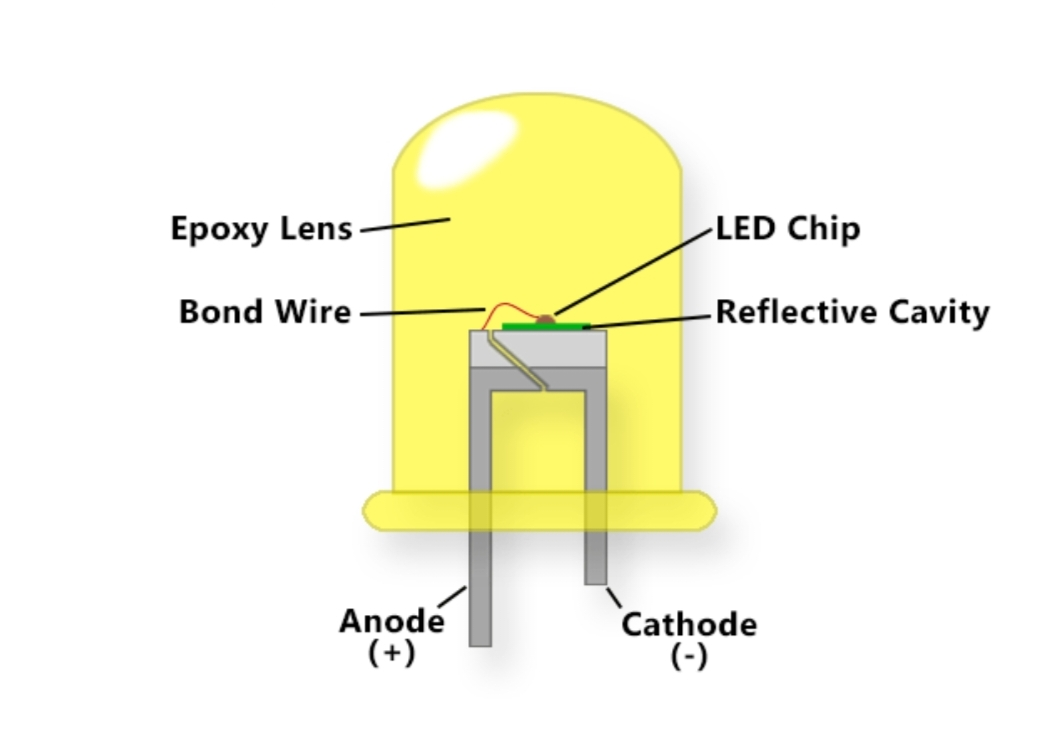
\includegraphics[width=0.4\textwidth]{ /storage/emulated/0/vignan/IMG_20241022_120046.jpg      }                         
	\caption{\label{fig-1:Gates}} 
	\end{figure}










\item Give two inputs called $x$ and $y$ seperately in bread board and make short connections of inputs and vcc and gnd.

\item By providing proper inputs observe the blinking of led for output $1$ and $0$ as per below truth table of xor operation.

	\begin{table} [htbp]
		\centering
\begin{tabular}{|c|c|c|}\hline
x & y & x $\oplus$ y \\\hline
0 & 0 & 0  \\ \hline
0 & 1 & 1 \\ \hline
1 & 0 & 1 \\ \hline
1 & 1 & 0 \\ \hline
\end{tabular}
		\vspace{0.1cm}
		\caption{\label{tab:widgets}}
	\end{table}



\item Execute the avr-gcc code in nvim editor using make command.
\item After upload the code into hardware setup using arduino IDE platform with .hex file.
 \end{enumerate}

\section{RESULTS}
 \begin{enumerate}
\item Download the codes given in the link below and execute them to see the output as shown in figure 2.
\item https://github.com/BynaboyinaAiswarya/Fwc-/blob/main/Avr-gcc/main.c
 \end{enumerate}


 \begin{figure}[h]                           
\centering                                 
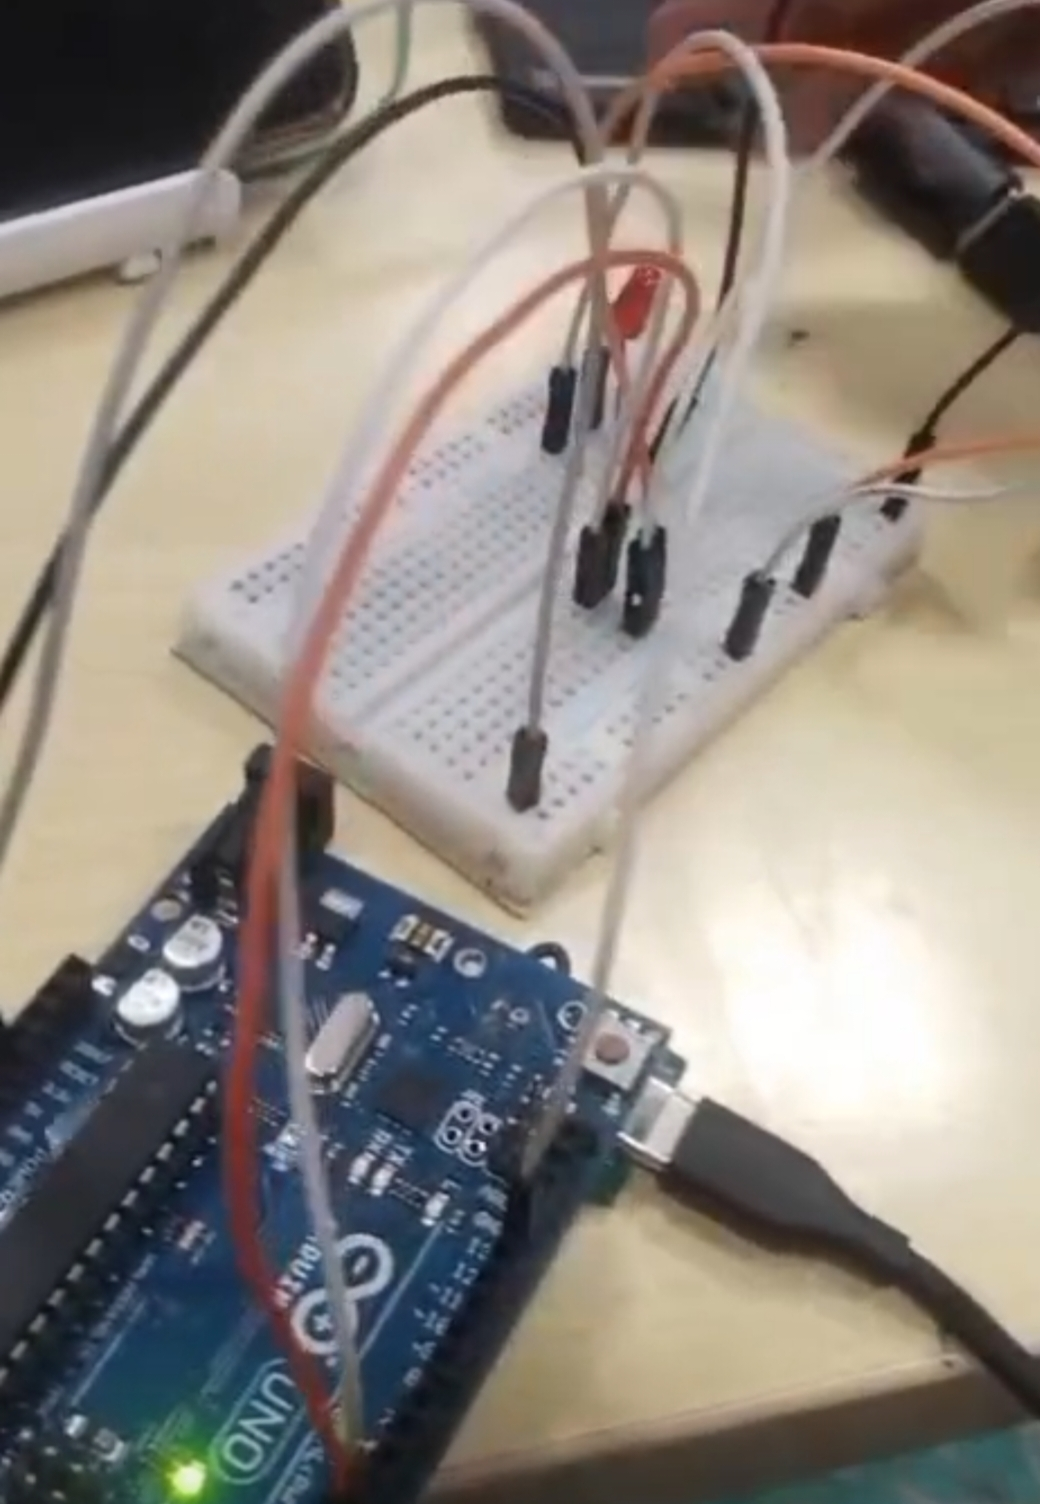
\includegraphics[width=0.4\textwidth]{  /storage/emulated/0/vignan/IMG_20241022_122001.jpg    }                                           
\caption{\label{fig-2:Gates}}               
\end{figure}
\section{CONCLUSION}
Hence implementation of avr-gcc code in arduino uno and the verification of xor truth tabe is done using led.


\end{document}
